% Document class 
\documentclass{article}

% Load this packages
\usepackage[process=auto]{external-inkscape}
\usepackage[process=auto]{external-matlab}
\usepackage[process=auto]{external-tikz}

% Load other packages
\usepackage{graphicx,import,color,subfigure,url,verbatim,pgfplots,csquotes}

% Define options for pgfplot
\pgfplotsset{compat=newest}
\pgfplotsset{plot coordinates/math parser=false}

\newlength\figurewidth \setlength\figurewidth{5cm}
\newlength\figureheight\setlength\figureheight{4cm}

% Prevent warnings for missing fonts
\let\otextbackslash\textbackslash
\renewcommand\textbackslash{{\rmfamily\otextbackslash}}
\let\otextbraceright\textbraceright
\renewcommand\textbraceright{{\rmfamily\otextbraceright}}
\let\otextbraceleft\textbraceleft
\renewcommand\textbraceleft{{\rmfamily\otextbraceleft}}

% Define title and author
\title{The externals packages}
\author{Andreas Kl\"ockner}
\date{\today}

% A command to display a tilde
\def\tttilde{\raise.17ex\hbox{$\scriptstyle\mathtt{\sim}$}}


% Begin document
\begin{document}
\maketitle


%%%%%%%%%%%%%%%%%%%%%%%%%%%%%%%%%%%%
% The Package                      %
%%%%%%%%%%%%%%%%%%%%%%%%%%%%%%%%%%%%
\section{Introduction}

The packages \texttt{external-inkscape} and \texttt{external-matlab} can be used to seamlessly import SVG and FIG images into latex documents. Figure \ref{fig:example} shows an example of a figure, which has been created with Inkscape. The left figure is exported from Inkscape. The right figure is imported with this package. You can see the compiled formula and the correct fonts.

\begin{figure}[h!]%
  \centering%
  \hfill
  \subfigure[As seen in Inkscape]{%
    \framebox{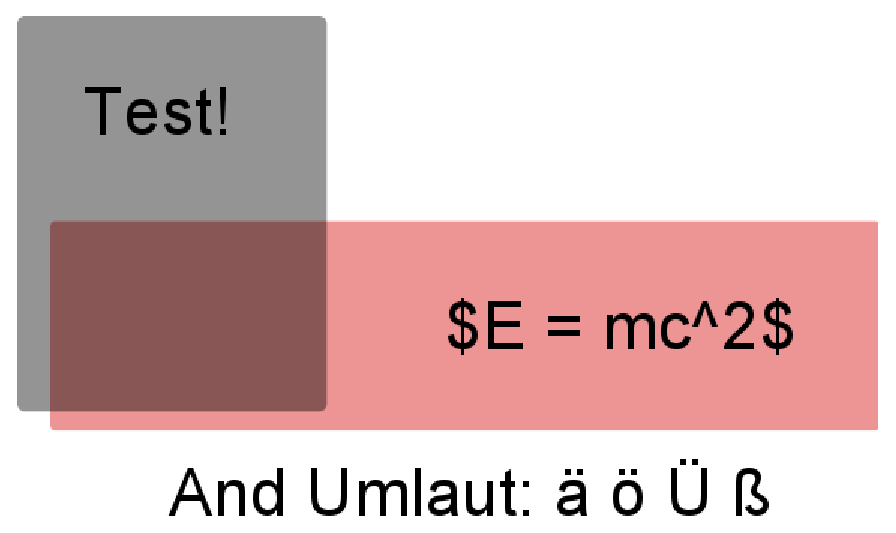
\includegraphics[width=5cm]{external-inkscape-example-raw}}}%
  \hfill
  \subfigure[Import via external-inkscape]{%
    \framebox{\includesvg[width=5cm]{external-inkscape-example}}}%
  \hfill\hbox{}
\caption{Example figure created in inkscape}%
\label{fig:example}%
\end{figure}


%%%%%%%%%%%%%%%%%%%%%%%%%%%%%%%%%%%%
% Package Usage                    %
%%%%%%%%%%%%%%%%%%%%%%%%%%%%%%%%%%%%
\section{The \texttt{external-base} package}
This package is used by the other packages in this collection. It checks for the correct options being set and provides some commands. The package only works inside the \emph{pdflatex compiler with the "-shell-escape" option enabled}!

\subsection{Command: \texttt{\textbackslash execute}}
The command \texttt{\textbackslash execute\{command\}} executes a shell command in the current working directory. It makes sure, the directory is used, even if it is UNC path name. This is done using th pushd command. If you use UNC paths, it appears normal, that the package \texttt{ifplatform} issues a warning. You should be fine to ignore it.

\subsection{Command: \texttt{\textbackslash executeiffilenewer}}
The command \texttt{\textbackslash executeiffilenewer\{source\}\{destination\}\{command\}} executes a shell command only if the \texttt{source} file is newer than the \texttt{destination} file.



%%%%%%%%%%%%%%%%%%%%%%%%%%%%%%%%%%%%
% Package Usage                    %
%%%%%%%%%%%%%%%%%%%%%%%%%%%%%%%%%%%%
\section{The \texttt{external-config} package}
This package allows external configuration for arbitrary other packages.

\subsection{Package loading}
The package should typically be used by package authors. It can be loaded using \texttt{\textbackslash RequirePackage\{external-config\}}. This defines two user commands described below.

\subsection{Command: \texttt{\textbackslash get@config}}
The command \texttt{\textbackslash get@config[<some file>]\{<some tag>\}} is meant to be used inside the custom package. It requests the \texttt{<some file>} to be read and executed. The \texttt{<some file>} can be edited by the end user to hold all installation-specific configuration, such as paths. If the \texttt{<some file>} is not set, it defaults to \texttt{external-config.conf}. The file may be located anywhere in the path. If the file does not exist, no additional configuration is set. Make sure, you have proper defaults set before calling \texttt{\textbackslash get@config}. 

Different classes of configuration can reside in the same \texttt{<some file>}. They can be marked with \texttt{<some tag>}. Any content in the \texttt{<some file>}, which is marked with the wrong \texttt{<some tag>} is ignored during the call to \texttt{\textbackslash get@config}. The markings are set by the user with \texttt{\textbackslash set@config} as described below. A typical \texttt{<some tag>} would be the package name.

\subsection{Command: \texttt{\textbackslash set@config}}
The command \texttt{\textbackslash set@config\{<some tag>\}\{<config commands>\}} executes the \texttt{<config commands>}, if the configuration for \texttt{<some tag>}
was requested by \texttt{\textbackslash get@config}. This command goes into the external configuration file \texttt{<some file>}.



%%%%%%%%%%%%%%%%%%%%%%%%%%%%%%%%%%%%
% Package Usage                    %
%%%%%%%%%%%%%%%%%%%%%%%%%%%%%%%%%%%%
\section{The \texttt{external-inkscape} package}
This procedure has been proposed by Johan B. C. Engelen in July 2010. You can see the original documentation here: \url{http://www.ctan.org/tex-archive/info/svg-inkscape}. Please keep in mind, that this package \emph{requires Inkscape version 0.48 or higher}!

\subsection{Package loading}
Use the \texttt{\textbackslash usepackage\{external-inkscape\}} command to load the package. 

\subsection{Package option: \texttt{path}}
You can set the path to your inkscape executable by specifying the \texttt{path} option to the package. This is not necessary, if inkscape is already on your search path.

\subsection{Package option: \texttt{process}}
By default, the included SVG images are only reprocessed when necessary, i.e. when the intermediate PDF is missing or older than the original SVG file. This can be deactivated by specifying the option \texttt{process=none}. If you want \texttt{external-inkscape} to pass over all images in the document, specify the option \texttt{process=all}.

\subsection{Package option: \texttt{changecatcodes}}
By default, all text in the SVG image is interpreted by \LaTeX. This includes special characters, such as \_ and \$. If you want to import these characters literally, you need to specify the package option \texttt{changecatcodes=true}. If you forget this, the imported \texttt{.pdf\_tex} file will throw \LaTeX\ errors, such as "missing \$".

\subsection{User command: \texttt{\textbackslash PathToInkscape\{\{pathto/inkscape\}\}}}
Apart from the package option you can use the \texttt{\textbackslash PathToInkscape} command to set your inkscape path.

\subsection{User command: \texttt{\textbackslash includesvg[options]\{filename\}}}
You can include an SVG image by issuing \texttt{\textbackslash includesvg[options]\{filename\}}. This will automatically convert and input the file \texttt{filename.svg}. If you want to define the size of the figure, you can do so by using the key-value syntax with the options \texttt{width}, \texttt{height} and \texttt{scale}.

\subsection{User command: \texttt{\textbackslash includesvg*} and \texttt{\textbackslash includesvg!}}
The starred variant of the \texttt{\textbackslash includesvg} command forces the conversion of the SVG file to the PDF file, even if the file has not been altered. The exclamation mark variant suppresses the conversion, even if the file has been altered. The use of these suffixes is overridden by the \texttt{process} option! This behavior is consistent with the one of the \texttt{pstool} package.

\subsection{Configuration file: \texttt{external-config.conf}}
This packages uses the \texttt{external-config} package to define inter-document settings for an installation. If you place a file named \texttt{external-config.conf} in your search path, this file will be read after loading the \texttt{external-inkscape} package, but before executing any options. The search path especially includes your RM\_LaTeX installation folder and the current working directory. Use \texttt{\textbackslash set@config\{external-inkscape\}\{<config commands>\}} to define your \texttt{external-inkscape} settings. It is suggested to put one \texttt{external-config.conf} file in your RM\_LaTeX installation directory, with your \texttt{\textbackslash PathToInkscape}: \\\\
\texttt{\textbackslash set@config\{external-inkscape\}\{ \\ 
\textbackslash PathToInkscape\{path/to/inkscape.exe\}\}}


\subsection{Example}
The following example illustrates the usage of the package:

\begin{verbatim}
\usepackage[path=path/to/inkscape]{external-inkscape}
...
\begin{figure}
  \includesvg[width=5cm]{external-inkscape-example}
\end{figure}
\end{verbatim}



%%%%%%%%%%%%%%%%%%%%%%%%%%%%%%%%%%%%
% Matlab                           %
%%%%%%%%%%%%%%%%%%%%%%%%%%%%%%%%%%%%
\section{The \texttt{external-matlab} package}
The \texttt{external-matlab} package has interfaces similar to the \texttt{external-inkscape} package. The commands are named \texttt{\textbackslash includefig}. There also are the variants \texttt{\textbackslash includefig*} and \texttt{\textbackslash includefig!}, which behave exactly as expected from the \texttt{external-inkscape} package.

The package also supports the options \texttt{path} and \texttt{process} as well the user command \texttt{\textbackslash PathToMatlab}. You can also use the \texttt{external-config.conf} configuration file to globally define the \texttt{\textbackslash PathToMatlab}. All configuration must be put in a \texttt{\textbackslash set@config\{external-matlab\}\{<config commands>\}} section: \\\\
\texttt{\textbackslash set@config\{external-matlab\}\{ \\ 
\textbackslash PathToMatlab\{path/to/matlab.exe\}\}}

\subsection{Example}
Figure \ref{fig:example:fig} shows an example, which has been imported using this package. Take care, that the options passed to \texttt{\textbackslash includefig} will only take effect, if the figure is reprocessed. Use \texttt{\textbackslash includefig*} once to ensure this.

\begin{figure}[ht]%
  \centering%
  \includefig[width=10cm]{external-matlab-example}%
	\caption{Example figure created in Matlab}%
	\label{fig:example:fig}%
\end{figure}

\subsection{Matlab over VPN connection}
To use matlab over vpn-connection, e.g. from home, you have to change the \texttt{\textbackslash PathToMatlab}. It is sufficient to insert the new path setting at the beginning of your document:
\begin{verbatim}
\PathToMatlab{matlab -c 27000@129.247.189.55}
\end{verbatim}
If it does not work out of the box, it might be due to the fact that the vpn-client is not connected. If you are at the institute, you need to be connected with the vpn-client as well in order to get a license with the changed path settings.

%%%%%%%%%%%%%%%%%%%%%%%%%%%%%%%%%%%%
% TikZ                             %
%%%%%%%%%%%%%%%%%%%%%%%%%%%%%%%%%%%%
\section{The \texttt{external-tikz} package}
\subsubsection*{(by Andreas Knoblach)}
The \texttt{external-tikz} package provides the command \texttt{\textbackslash includetikz}, which allows to create a pdf from a TikZ figure and to include this pdf file.  This helps to improve the compilation time for documents including complex TikZ figures. The TikZ figure has to be defined in a separate tex file. Again, the two variants \texttt{\textbackslash includetikz*} and \texttt{\textbackslash includetikz!} are provided. Additionally, the command \texttt{\textbackslash includetikz\tttilde} will cause that TikZ code is directly included. Finally, \texttt{\textbackslash includetikz=} does the same like \texttt{\textbackslash includetikz\tttilde} but it cannot be overridden by the package's process option.

Similar to the \texttt{pstool} package, \texttt{external-tikz} must detect the end of the preamble. Since this is not always possible, \texttt{\textbackslash EndPreamble} can be used to mark the end of the preamble.

\subsection{Package Options}
The package also supports the options \texttt{process} like the \texttt{external-inkscape}. In addition to the values  \texttt{auto}, \texttt{all}, and \texttt{none}, \texttt{process=tikz} can be used to include the TikZ code directly of all \texttt{\textbackslash includtikz} figures. Creating complex figure might cause a \enquote{TeX capacity exceeded} error. In this cases, the package option \texttt{lua} can be used and the figure is created using LuaLaTeX. Because LuaLaTeX can use the complete RAM, a \enquote{TeX capacity exceeded} error is unlikely. Note that, although the most packages work well with LuaLaTeX, there are some incompatibilities.

The option \texttt{cleanup} can be used to specify which temporary files shall be deleted. The default ones are \texttt{.log}, \texttt{.tex} and \texttt{.aux}; this corresponds to the package options \texttt{cleanup=\{.log,.tex,.aux\}}.

\subsection{Example}
Figure \ref{fig:example:tikz} shows an example, which has been imported using this package.
\begin{figure}[ht]%
	\centering
	\includetikz{external-tikz-example}
	\caption{Example figure included using external-tikz}
	\label{fig:example:tikz}
\end{figure}



%%%%%%%%%%%%%%%%%%%%%%%%%%%%%%%%%%%%
% Installation                     %
%%%%%%%%%%%%%%%%%%%%%%%%%%%%%%%%%%%%
\section{Installation}
\begin{enumerate}
	\item Make sure, you have Inkscape version 0.48 or higher.
	\item Copy the package to any desired path. It is important that you do not change the directory structure.
	\item Open the MikTeX Settings GUI and add the package path to the MikTeX root directory list.
	\item You may need to refresh the filename database (FNDB).
	\item Use the pdflatex compiler with the "-shell-escape" option.
\end{enumerate}




%%%%%%%%%%%%%%%%%%%%%%%%%%%%%%%%%%%%
% Issues                           %
%%%%%%%%%%%%%%%%%%%%%%%%%%%%%%%%%%%%
\section{Troubleshooting}
\begin{enumerate}
	\item Make sure, you have Inkscape version 0.48 or higher. \\
	      Only like this can you take advantage of its new pdf\_tex export function.
	\item Use the pdflatex compiler with the "-shell-escape" option. \\
	      This enables latex to automatically trigger the conversion.
	\item This package also uses the \texttt{graphicx}, \texttt{color}, \texttt{import}, \texttt{xkeyval}, \texttt{calc} and \texttt{suffix} packages.
	\item If you use UNC paths, it appears normal, that the package \texttt{ifplatform} issues a warning. You should be fine to ignore it.
	\item If you receive warnings about missing \$ characters, you should use the \texttt{changecatcode=true} option of the \texttt{external-inkscape} package.
	\item If your configuration files are not processed, you might need to refresh the filename database of your MikTeX installation.

\end{enumerate}





\end{document}
% eof
